\documentclass[11pt]{article}
\usepackage[margin=1.15in]{geometry}
\usepackage{amsmath,amssymb,amsthm}
\usepackage{graphicx}
\usepackage{booktabs}
\usepackage{xcolor}
\usepackage[colorlinks=true,linkcolor=blue!60!black,citecolor=blue!60!black,urlcolor=blue!60!black]{hyperref}

\newtheoremstyle{itheads}{\topsep}{\topsep}{}{}{\itshape}{.}{.5em}{}
\theoremstyle{itheads}
\newtheorem{theorem}{Theorem}
\newtheorem{proposition}{Proposition}
\newtheorem{lemma}{Lemma}
\newtheorem{corollary}{Corollary}

\newcommand{\E}{\mathbb{E}}
\newcommand{\R}{\mathbb{R}}
\newcommand{\sech}{\operatorname{sech}}
\newcommand{\artanh}{\operatorname{artanh}}

\title{A Proof That the Grass Is Greener\\[4pt]
{\large Three-shot search on an exponentiated Ornstein--Uhlenbeck landscape}}
\author{Peter Cotton}
\date{\normalsize First version: April 6, 2022. This version: September 3, 2026.}

\begin{document}
\maketitle

\begin{abstract}
\noindent A searcher evaluates a rugged landscape --- the exponential of an
Ornstein--Uhlenbeck path --- at three points chosen sequentially, and is
paid the value at the final point. The two-evaluation problem has a
three-phase closed form: flee somewhere fresh if the first value is below
the median, stay put if it is exceptional, and otherwise step a distance
set by the mean-reversion scale. The interesting question is the third
evaluation: given two locations a bracket apart, should the searcher ever
place the final point between them? A rapidity coordinate
$\theta=\artanh(e^{-\kappa\,\Delta t})$, under which bridge means compose
additively, reduces the comparison to a hyperbolic identity: an interior
bridge point has the same conditional mean as the outside point at the
composed rapidity and conditional variance larger by the factor
$\cosh(\theta_2+\theta)/\cosh(\theta_2-\theta)$. Since the objective
rewards variance, the interior point beats its mean-matched outside
rival everywhere except at the bracket's ends. Against the best outside
choice the interior wins precisely for anchor values $b$ between a
closed-form quadratic root and $e^{2\Theta}=(1+\rho)/(1-\rho)$, with
$\rho$ the bracket correlation and $\Theta$ its rapidity: stay between
the anchors on good news; on bad news step out past the better end,
whichever end that is. Within the region the optimal interior point is
the bracket middle only up to $b=\sinh 2\tau$, $\tau$ the half-bracket
rapidity; beyond, a pitchfork sends a mirror pair of optima sliding
toward the ends, which they reach exactly at the region's upper edge.
Numerically, the optimal three-shot policy widens the
bracket relative to the two-shot step in anticipation of the revisit
option, which is worth up to about one percent of expected value. In
every phase of the policy the winning location is one never yet
visited: under a lognormal objective an unvisited point with the same
expected height as a visited one is strictly better, by Jensen's
inequality, so the grass provably is greener --- the searcher's only
question is where it is greenest.
\end{abstract}

\section{The problem: three evaluations of an exponentiated OU path}

Let $X$ be a stationary Ornstein--Uhlenbeck process on $\R$ with
$\E[X_t]=0$, unit marginal variance, and covariance kernel
\begin{equation}
k(s,t) \;=\; e^{-\kappa|s-t|}.
\end{equation}
The landscape is $f(t)=\exp(X_t)$: locally continuous, mean-reverting in
its logarithm, with occasional high peaks where excursions are magnified
by the exponential. A searcher samples $f$ at a first location, which we
take to be $t_0=0$ by translation invariance, discovering $X_0=b$. Two
further evaluations at locations $t_1$ and then $t_2$ follow, each chosen
with knowledge of all values so far, and the payoff is the value at the
final location,
\begin{equation}
u \;=\; \E\!\left[f(t_2)\right]
\;=\; \E\!\left[e^{X_{t_2}}\right].
\end{equation}
Since $X_{t_2}$ is conditionally Gaussian given the observations, with
mean $\mu$ and variance $\nu$ depending on the chosen location,
\begin{equation}\label{eq:lognormal}
\log \E\!\left[e^{X_{t_2}}\right] \;=\; \mu + \tfrac{1}{2}\nu ,
\end{equation}
and the searcher is paid for conditional mean and conditional variance in
equal measure. This is the engine of everything below: exploration has
value not only through what it might reveal along the way but directly,
because a final location with residual uncertainty carries a lognormal
bonus of half its variance.

Two conventions tidy the boundary cases. A searcher may take a location
to infinity, which by mean reversion is equivalent to sampling a fresh
$N(0,1)$ value independent of everything seen; and a searcher may revisit
an existing location, receiving its known value. Neither changes the
substance of any result.

\section{Two evaluations: flee, explore, or stay}

Given only $X_0=b$, a candidate second location at distance $t$ has
$X_t \sim N\!\left(b\lambda,\,1-\lambda^{2}\right)$ with
$\lambda=e^{-\kappa t}\in(0,1]$. From \eqref{eq:lognormal},
\begin{equation}
\log \E\!\left[e^{X_t}\right]
\;=\; b\lambda + \tfrac{1}{2}\!\left(1-\lambda^{2}\right)
\;=\; -\tfrac{1}{2}\left(\lambda-b\right)^{2} + \tfrac{1}{2}\left(b^{2}+1\right),
\end{equation}
maximized over $\lambda\in[0,1]$ at $\lambda^{*}=\min\{\max\{b,0\},1\}$.
Three phases result.

\begin{proposition}[Two-shot policy]\label{prop:twoshot}
The optimal second location and its log-value $\zeta(b)$ are
\begin{equation}
t^{*} \;=\;
\begin{cases}
\infty & b<0 \quad(\text{flee}),\\[2pt]
-\tfrac{1}{\kappa}\log b & 0\le b\le 1 \quad(\text{explore}),\\[2pt]
0 & b>1 \quad(\text{stay}),
\end{cases}
\qquad
\zeta(b) \;=\;
\begin{cases}
\tfrac{1}{2} & b<0,\\[2pt]
\tfrac{1}{2}\left(b^{2}+1\right) & 0\le b\le 1,\\[2pt]
b & b>1 .
\end{cases}
\end{equation}
\end{proposition}

A below-median first value is abandoned entirely; an exceptional one is
kept; in between, the searcher steps to the distance at which the prior
pull toward the anchor exactly matches the anchor's height. The value
$\zeta$ will serve as the outside benchmark throughout. Outside the
bracket means either ray, and by the Markov property an outside point
sees only its nearest anchor, so the best outside move steps past
whichever end is better --- reversing direction, when the second value
disappoints, to leave by the first anchor rather than the second.
There is no momentum in the policy; only the heights of the ends
matter.

\section{Bridge moments and the rapidity coordinate}

Now suppose values $X_0=b$ and $X_{t_1}=d$ are known, and write
$\rho=e^{-\kappa t_1}$ for the bracket correlation. For an interior
location $t_2\in(0,t_1)$ let $\lambda_2=e^{-\kappa t_2}$ and
$\lambda=e^{-\kappa(t_1-t_2)}$ be the correlations to the two ends, so
$\lambda_2\lambda=\rho$. Gaussian conditioning gives the bridge moments
\begin{equation}\label{eq:bridge}
\mu \;=\; \frac{\lambda_2\!\left(1-\lambda^{2}\right)b
+ \lambda\!\left(1-\lambda_2^{2}\right)d}{1-\rho^{2}},
\qquad
\nu \;=\; \frac{\left(1-\lambda_2^{2}\right)\left(1-\lambda^{2}\right)}
{1-\rho^{2}} .
\end{equation}
The bridge sags: for $b=d>0$ the mean is below $b$ everywhere strictly
inside, pulled toward the process mean, while the variance rises from
zero at the ends to a maximum at the middle.

Define rapidities
\begin{equation}
\theta_2 = \artanh(\lambda_2), \qquad \theta = \artanh(\lambda),
\end{equation}
so named because, in the symmetric case $d=b$, bridge means compose like
relativistic velocities:
\begin{equation}\label{eq:meanadd}
\mu \;=\; b\,\frac{\lambda_2+\lambda}{1+\lambda_2\lambda}
\;=\; b\tanh\!\left(\theta_2+\theta\right).
\end{equation}
The variance in \eqref{eq:bridge} also takes a hyperbolic product form.
Substituting $1-\tanh^{2}=\sech^{2}$ and using
$\cosh(A+B)\cosh(A-B)=\cosh^{2}\!A\cosh^{2}\!B-\sinh^{2}\!A\sinh^{2}\!B$,
\begin{equation}\label{eq:varprod}
\nu \;=\; \frac{\sech^{2}\theta_2\,\sech^{2}\theta}
{1-\tanh^{2}\theta_2\tanh^{2}\theta}
\;=\; \sech\!\left(\theta_2+\theta\right)\sech\!\left(\theta_2-\theta\right).
\end{equation}
An outside location beyond $t_1$ at correlation
$\lambda'=\tanh\theta'$ to its anchor has, by the Markov property, mean
$d\tanh\theta'$ and variance
\begin{equation}\label{eq:outvar}
1-\tanh^{2}\theta' \;=\; \sech^{2}\theta' .
\end{equation}

\section{Interior points beat their mean-matched outside rivals}

Equations \eqref{eq:meanadd}--\eqref{eq:outvar} settle the comparison
between an interior point and the outside point engineered to match its
mean.

\begin{theorem}[Bridge dominance]\label{thm:dominance}
Let $d=b$ and let $t_2\in(0,t_1)$ be an interior location with
rapidities $(\theta_2,\theta)$. The outside location at composed
rapidity $\theta'=\theta_2+\theta$ has the same conditional mean
$b\tanh(\theta_2+\theta)$, and the ratio of conditional variances is
\begin{equation}
\frac{\nu_{\mathrm{inside}}}{\nu_{\mathrm{outside}}}
\;=\; \frac{\sech(\theta_2+\theta)\sech(\theta_2-\theta)}
{\sech^{2}(\theta_2+\theta)}
\;=\; \frac{\cosh(\theta_2+\theta)}{\cosh(\theta_2-\theta)} \;\ge\; 1,
\end{equation}
with equality only in the degenerate limits $\theta_2\to\infty$ or
$\theta\to\infty$ (the bracket's ends). By \eqref{eq:lognormal} the
interior point's utility is at least that of its mean-matched outside
rival, strictly so in the interior, for every anchor value $b$.
\end{theorem}

\begin{proof}
The mean statement is \eqref{eq:meanadd} against the outside mean
$b\tanh\theta'$ at $\theta'=\theta_2+\theta$; the variance ratio is
\eqref{eq:varprod} against \eqref{eq:outvar}; and
$\cosh(\theta_2+\theta)\ge\cosh(\theta_2-\theta)$ with equality iff
$\theta_2\theta=0$. Utility \eqref{eq:lognormal} is increasing in $\nu$
at fixed $\mu$.
\end{proof}

The interior of a bracket whose two ends are both worth $b$ is,
point for point, a better bet than the outside locations with the same
expected height: the bridge keeps most of the anchors' mean while
retaining, at its middle, variance
$\sech(\theta_2+\theta)$ against the outside's
$\sech^{2}(\theta_2+\theta)$ --- up to three times as much residual
uncertainty at the same expectation, and the objective pays for
uncertainty.

\section{The exact revisit region, and a pitchfork inside it}

Dominance over mean-matched rivals does not by itself decide the
searcher's move, because the outside player is free to choose any
correlation. The relevant comparison is the best interior point
against the best outside value $\zeta$ of
Proposition~\ref{prop:twoshot}, and it requires knowing where the
interior optimum sits. It is not always the middle.

\begin{theorem}[Interior critical points, symmetric case]\label{thm:pitchfork}
For $d=b>0$ write the interior log-utility as a function of the
correlation $x=\lambda_2\in(\rho,1)$ to one end,
\begin{equation}
f(x) \;=\; \frac{b\left(x+\rho/x\right)}{1+\rho}
+ \frac{\left(1-x^{2}\right)\left(1-\rho^{2}/x^{2}\right)}{2\left(1-\rho^{2}\right)}.
\end{equation}
Its critical points solve
\begin{equation}\label{eq:factor}
\left(x^{2}-\rho\right)\left(x^{2}-b\left(1-\rho\right)x+\rho\right)\;=\;0 .
\end{equation}
The middle $x=\sqrt{\rho}$ is always critical. Writing
$\tau=\artanh\sqrt{\rho}$ for the half-bracket rapidity, the middle
is the interior optimum if and only if
\begin{equation}
b \;\le\; \sinh 2\tau \;=\; \frac{2\sqrt{\rho}}{1-\rho},
\end{equation}
at which threshold a pitchfork bifurcation occurs: for
$b>\sinh 2\tau$ the middle is a local minimum and the optimum is the
mirror pair
\begin{equation}\label{eq:offmid}
x_{\pm} \;=\; \frac{b\left(1-\rho\right)
\pm\sqrt{b^{2}\left(1-\rho\right)^{2}-4\rho}}{2},
\qquad x_{+}x_{-}=\rho,
\end{equation}
one point seen from each end. The pair is born at the middle and
migrates outward, reaching the ends exactly at
$b=\left(1+\rho\right)/\left(1-\rho\right)=e^{2\Theta}$, where
$\Theta=\artanh\rho$ is the full-bracket rapidity.
\end{theorem}

\begin{proof}
The interior problem is secretly one-dimensional in
$\sigma = x + \rho/x = \lambda_2+\lambda$, under which mirror points
coincide: using $\left(1-x^{2}\right)\left(1-\rho^{2}/x^{2}\right)
= \left(1+\rho\right)^{2}-\sigma^{2}$,
\begin{equation}\label{eq:parabola}
f \;=\; \frac{b\,\sigma}{1+\rho}
+ \frac{\left(1+\rho\right)^{2}-\sigma^{2}}{2\left(1-\rho^{2}\right)},
\end{equation}
a downward parabola in $\sigma$ with peak at
$\sigma^{*}=b\left(1-\rho\right)$, while $\sigma$ ranges over
$[\,2\sqrt{\rho},\,1+\rho)$ --- its minimum at the middle, its
supremum at the ends. Since $d\sigma/dx = 1-\rho/x^{2}$ vanishes only
at the middle, the critical points of $f$ are the middle together
with the preimages of $\sigma^{*}$, which lie in range iff
$2\sqrt{\rho} < b\left(1-\rho\right) < 1+\rho$; solving
$x+\rho/x=b\left(1-\rho\right)$ gives \eqref{eq:offmid} and, with the
middle factor, \eqref{eq:factor}. The middle sits at the
$\sigma$-minimum, so it is the interior optimum iff the parabola is
decreasing there, $\sigma^{*}\le 2\sqrt{\rho}$, i.e.
$b\le 2\sqrt{\rho}/\left(1-\rho\right)
= 2\tanh\tau\cosh^{2}\tau=\sinh 2\tau$; beyond, the peak itself is
attained by the mirror pair, and $x_{+}=1$ exactly when
$\sigma^{*}=1+\rho$, i.e. $b=e^{2\Theta}$.
\end{proof}

\begin{corollary}[Off-middle value]\label{cor:uoff}
For $\sinh 2\tau \le b \le e^{2\Theta}$ the interior optimum equals
the parabola's peak value,
\begin{equation}\label{eq:uoff}
U_{\mathrm{off}}(b,\rho) \;=\;
\tfrac12\!\left(b^{2}e^{-2\Theta} + e^{2\Theta}\right),
\end{equation}
obtained by substituting $\sigma^{*}=b\left(1-\rho\right)$ into
\eqref{eq:parabola} and using $e^{2\Theta}=(1+\rho)/(1-\rho)$.
\end{corollary}

The searcher on very good news does not aim for the center of the
bracket: the optimal patch slides from the middle toward the
better-known ends as the anchors improve, hugging them ever more
closely, and merges with them exactly when $b$ reaches $e^{2\Theta}$.

\begin{theorem}[Revisit region, symmetric case]\label{thm:boundary}
For $d=b\ge 0$ the best interior point strictly beats every outside
location precisely for
\begin{equation}\label{eq:region}
b_{-}(\rho) \;<\; b \;<\; \frac{1+\rho}{1-\rho} \;=\; e^{2\Theta},
\qquad
b_{-}(\rho)=\frac{\sqrt{\rho}\left(2-\sqrt{2\left(1-\rho\right)}\right)}{1+\rho}.
\end{equation}
The lower edge is the smaller root of
$b^{2}\left(1+\rho\right)-4b\sqrt{\rho}+2\rho=0$, the middle-regime
comparison $U_{\mathrm{mid}}=\zeta$ with
$U_{\mathrm{mid}}(b,\rho)=2b\sqrt{\rho}/(1+\rho)
+\left(1-\rho\right)/\left(2\left(1+\rho\right)\right)$; the upper
edge is where the off-middle optima \eqref{eq:offmid} reach the
bracket's ends.
\end{theorem}

\begin{proof}
Everything reduces to the parabola \eqref{eq:parabola} and three
regimes of its peak. If $b\ge e^{2\Theta}$ then
$\sigma^{*}\ge 1+\rho$: $f$ increases in $\sigma$ over the whole
range, its supremum is the unattained end limit $b$, and staying
wins. If $\sinh 2\tau < b < e^{2\Theta}$ the optimum is
$U_{\mathrm{off}}$ of Corollary~\ref{cor:uoff}, and both comparisons
are one line: for $b>1$,
\begin{equation}
U_{\mathrm{off}} - b \;=\;
\tfrac12\,e^{-2\Theta}\!\left(b-e^{2\Theta}\right)^{2} \;>\;0,
\end{equation}
the arithmetic--geometric mean inequality applied to the two terms
of \eqref{eq:uoff}, with equality only at the tangency
$b=e^{2\Theta}$ that defines the upper edge; and for $b\le 1$,
\begin{equation}
U_{\mathrm{off}} - \tfrac12\!\left(b^{2}+1\right) \;=\;
\tfrac12\!\left(e^{2\Theta}-1\right)\!\left(1-b^{2}e^{-2\Theta}\right)
\;>\;0
\end{equation}
since $b\le 1<e^{\Theta}$. If $b\le\sinh 2\tau$ the optimum is the
middle. For $b\le 1$, $U_{\mathrm{mid}}>\zeta$ is the stated
quadratic; $b_{-}\le 2\sqrt{\rho}/\left(1+\rho\right)<\sinh 2\tau$
places the lower edge inside this regime, so it is exact. No gap
opens above: when $\sinh 2\tau\le 1$ (i.e.
$\rho\le 3-2\sqrt{2}$), $b_{+}\ge\sinh 2\tau$ reduces to
$\left(1-\rho\right)^{3}\ge 8\rho^{2}$, whose left side decreases
and right side increases in $\rho$ and which holds at
$\rho=3-2\sqrt{2}$; when $\sinh 2\tau>1$, $b_{+}\ge 1$ reduces, with
$u=\sqrt{\rho}$, to $2u^{2}\left(1+u\right)\ge\left(1-u\right)^{3}$,
increasing against decreasing and true at $u=\sqrt{2}-1$ (it reads
$20\sqrt{2}\ge 28$); and on $1<b\le\sinh 2\tau$,
$U_{\mathrm{mid}}\ge b$ reduces to
$b\le\left(1+u\right)/\left(2\left(1-u\right)\right)$, which covers
the whole stretch because $\sinh 2\tau\le
\left(1+u\right)/\left(2\left(1-u\right)\right)$ is
$\left(1-u\right)^{2}\ge 0$. Assembling the regimes, the interior
wins exactly on \eqref{eq:region}.
\end{proof}

Along the two-shot-inherited bracket $\rho=b$ the region opens at
$b^{*}=0.4233\ldots$, the root of $U_{\mathrm{mid}}(b,b)=\zeta(b)$.
Spot values with $\rho=b$: at $b=0.30$ the middle offers $0.5220$
against the outside $0.5450$ (go forth); at $b=0.50$, $0.6381$
against $0.6250$ (revisit); at $b=0.90$, $0.9251$ against $0.9050$
(revisit). By continuity the region extends to $d\ne b$: at $b=0.5$,
$\rho=0.5$ the interior wins for all $d\ge b$ and loses for
$d\le 0.45$. And notably the region reaches above $b=1$: even an
anchor better than the two-shot stay threshold is worth leaving for
a point just inside the bracket, provided $b<e^{2\Theta}$ --- wide
brackets forgive very good news.

\begin{figure}[t]
\centering
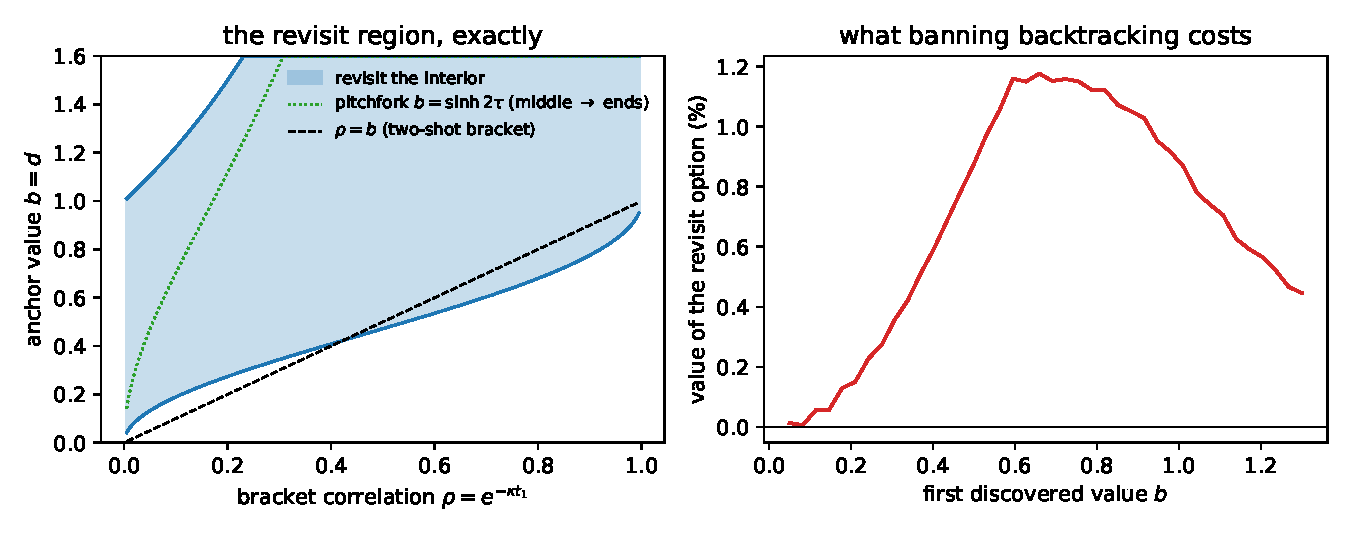
\includegraphics[width=\textwidth]{figures/phase.pdf}
\caption{Left: the exact symmetric revisit region
\eqref{eq:region} in the plane of bracket correlation $\rho$ and
anchor value $b=d$, bounded below by the quadratic root $b_{-}$ and
above by $e^{2\Theta}=\left(1+\rho\right)/\left(1-\rho\right)$. The
dotted curve is the pitchfork $b=\sinh 2\tau$: below it the optimal
interior point is the bracket middle, above it the mirror pair
\eqref{eq:offmid} hugging the ends. The dashed line is the two-shot
bracket $\rho=b$, entering the region at $b^{*}=0.4233$. Right: the
value of the revisit option --- the percentage increase in expected
payoff of the full three-shot optimum over the best policy forbidden
to backtrack --- as a function of the first discovered value $b$,
with the bracket optimized in both cases.}
\label{fig:phase}
\end{figure}

\section{The three-shot policy, computed}

The first location $t_1$ should anticipate the endgame. Writing
$V(b,d,\rho)$ for the best of the outside values
$\zeta(b),\zeta(d)$ and the interior optimum, the three-shot value of a
bracket $\rho$ is
$\log \E_d\!\left[e^{V(b,d,\rho)}\right]$ with
$d\sim N(b\rho,\,1-\rho^{2})$, evaluated by quadrature. Optimizing over
$\rho$ yields the policy. Three features, all visible in
Table~\ref{tab:threeshot} and Figure~\ref{fig:phase}:

\begin{table}[t]
\centering
\begin{tabular}{rcccc}
\toprule
$b$ & optimal $\rho$ & value & value, no revisit & revisit worth \\
\midrule
$-0.5$ & $\to 0$ & $0.8306$ & $0.8306$ & $0.00\%$ \\
$0.1$ & $0.06$ & $0.8398$ & $0.8394$ & $0.03\%$ \\
$0.3$ & $0.16$ & $0.8728$ & $0.8695$ & $0.33\%$ \\
$0.5$ & $0.28$ & $0.9392$ & $0.9304$ & $0.88\%$ \\
$0.7$ & $0.40$ & $1.0378$ & $1.0262$ & $1.16\%$ \\
$0.9$ & $0.50$ & $1.1670$ & $1.1567$ & $1.03\%$ \\
$1.2$ & $0.62$ & $1.4060$ & $1.4004$ & $0.56\%$ \\
\bottomrule
\end{tabular}
\caption{The three-shot game: optimal bracket correlation, log-value,
the log-value of the best policy forbidden to revisit the bracket
interior, and the percentage the revisit option adds to expected payoff.
Gauss--Hermite quadrature with $61$ nodes over the second value $d$;
interior optima on a $400$-point grid.}
\label{tab:threeshot}
\end{table}

First, a below-median start still means flight: for $b<0$ the optimal
bracket correlation tends to zero (the searcher abandons the anchor,
collecting fresh draws) and the revisit option is worthless, since a
bridge between an abandoned anchor and whatever follows is a bridge
between things not worth bridging.

Second, the optimal bracket is wider than the two-shot step. At
$b=0.5$ the two-shot policy steps to $\rho=0.5$; the three-shot optimum
stretches to $\rho=0.28$. The wide bracket is bought in anticipation of
the endgame: a wider bracket makes the eventual bridge middle more
uncertain, and \eqref{eq:lognormal} pays half of that uncertainty
directly.

Third, the revisit option's worth peaks near one percent of expected
value around $b\approx0.7$ and vanishes at both extremes --- worthless
when the start is abandoned, nearly worthless when the start is so good
the policy barely moves. Forbidding backtracking is thus a cheap
approximation by value, but it is not the optimal policy, and its
prescription is qualitatively wrong exactly when both evaluations came
in high.

\section{Discussion}

The proverb, read as mathematics, is Jensen's inequality: under a
payoff that exponentiates a Gaussian, any unvisited location whose
expected height matches a visited one is strictly better, carrying a
bonus of half its residual variance. The grass is greener --- provably,
not wistfully --- and the analysis above locates the greenest patch.
On bad news, leave: a below-median
anchor is abandoned outright, and a disappointing second value sends
the final point out past the better end --- in whichever direction
that end lies. On good news, stay between: when both ends
of the bracket came in high, the sagging bridge between them retains
most of their promise and, at its middle, several times the residual
uncertainty of any outside point with the same expectation --- and an
objective that exponentiates a Gaussian pays for uncertainty at
half-weight. The exact frontier between the two regimes is the
quadratic \eqref{eq:quadratic}.

A caution about the word exploration. With one evaluation remaining
there is nothing to explore: no discovery at the final point can
inform a later choice, because there is none. The last move is pure
placement --- put the point where $\mu+\tfrac12\nu$ is largest ---
and the pull toward uncertain locations is Jensen's inequality, not
curiosity: the objective pays half the variance directly, whether or
not anything is ever learned there. Exploration proper enters only
with more shots remaining, where early placements buy information. The
natural conjecture from the endgame here is a two-phase $k$-shot
policy: step out past the running best while values keep climbing,
each new high re-anchoring the next step, then refine between the two
highest once a good region is bracketed. Settling it is a dynamic program over the posterior, cheap
per step with the bridge formulas above.

The rapidity coordinate is the tool worth keeping: bridge means compose
additively in $\theta=\artanh(e^{-\kappa\Delta t})$, bridge variances
factor as $\sech(\theta_2+\theta)\sech(\theta_2-\theta)$, and the
inside--outside comparison collapses to the monotonicity of
$\cosh$. The same coordinate is the natural discretization for lattice
computations of extremes of OU paths, where uniform-in-$\theta$ spacing
makes correlations additive across cells.

Beyond three shots the closed forms give out, and the $k$-shot policy is
a dynamic program over the posterior --- bridge moments per interval,
maximization over intervals --- that the formulas here make cheap per
step. The landscapes themselves remain a useful synthetic test bed for
few-shot exploration algorithms: the choice between striking out and
revisiting is a one-bit probe of whether a search strategy has grasped the
trade between mean reversion and the variance bonus, and
\eqref{eq:quadratic} is the answer key.

\subsection*{Reproducibility}

All numbers and the figure are produced by
\texttt{numerics.py} alongside this source, with an independent
verification of Theorems~\ref{thm:dominance} and \ref{thm:boundary}
by exact conditioning and weighted Monte Carlo in
\texttt{verify/check\_inside.py}, in the
\href{https://github.com/microprediction/browniansearch}{browniansearch}
repository.

\begin{thebibliography}{9}

\bibitem{callander2011}
S.~Callander.
Searching for good policies.
\emph{American Political Science Review}, 105(4):643--662, 2011.

\bibitem{baumann2019}
O.~Baumann, J.~Schmidt, and N.~Stieglitz.
Effective search in rugged performance landscapes: a review and outlook.
\emph{Journal of Management}, 45(1):285--318, 2019.

\bibitem{grill2018}
J.-B. Grill, M.~Valko, and R.~Munos.
Optimistic optimization of a Brownian.
In \emph{Advances in Neural Information Processing Systems~31}, 2018.

\bibitem{calvin1997}
J.~M. Calvin.
Average performance of a class of adaptive algorithms for global
optimization.
\emph{Annals of Applied Probability}, 7(3):711--730, 1997.

\bibitem{agrawal1995}
R.~Agrawal.
The continuum-armed bandit problem.
\emph{SIAM Journal on Control and Optimization}, 33(6):1926--1951, 1995.

\end{thebibliography}

\end{document}
